
\chapter{Experiments}
\label{chap:Experiments} 

\section{Methods}

The success of the reconstruction largely depends on the representation of the data
after the feature-map is applied.
Although, assuming that the data distribution of the data can be accurately described
by a mean and a variance is a strong assumption.
More sophisticated ways of modeling data distributions exist
\XXX{insert some}
, yet mean and variance were chosen due to their simplicity in evaluation and computing of the gradients.

The feature-map will ideally "disentangle" the data space to enable 
simple statistics to capture the complexity of the data set.

It is hypothesized that neural networks "disentangle" the input space in order to end up with an efficient feature-representation in its later layers.
(This becomes more apparent when one imagines that most neural networks must learn to classify by linearly separating its features obtained from the previous to last layer.)


For assessing the efficacy of the ability to capture the data distribution by
the statistics of the intermediary representations in a neural network,
several different mappings or collections of mappings will be compared. 

For every method there exists a class-dependent variant.
\subsection{neural network}

A \textbf{neural network} $\Phi$ is a function that maps an input $\vec x \in \R^d$ to a label $y$.
Normally, in classification tasks, where one hopes to assign a label to an input, the output of a neural network is a C-dimensional vector..
\XXX{maybe not, logit; DEF}. 
A \textbf{multi-layer perceptron} (MLP) is a special type of neural network. Throughout this work, when referring to a neural network, a multi-layer perceptron is meant. A MLP is a composition of functions $\Phi_i$, also called \textbf{layers} that successively act on the outputs $\vec h$ of the previous layer, called \textbf{activations} or \textbf{hidden states}. 
The last layer is referred to as the \textbf{logits-layer}. 
The predicted output label $\hat y$ is normally obtained by returning the index of the maximum value in the logits-layer, thus $\R^{\textnormal L} = \R^C$.
In a plain \textbf{fully-connected} neural network, the layers are each made up of an affine linear transformation and a non-linear activation function.

Formally, a fully-connected neural network of layer depth L is described as:

\[
    \Phi = \Phi_\text{L} \circ \ldots \circ \Phi_1
\]
\[
    \vec h_\ell = (\Phi_\ell \circ \ldots \circ \Phi_1) (\vec x) =
    \Phi_\ell(\vec h_{\ell-1}) \in \R^{d_\ell}
\]
$\Phi_\ell$ then, is a mapping from $\R^{d_{\ell-1}}$ to $\R^{d_\ell}$. 
The space of a hidden state $\vec h$ is called a \textbf{feature-space}.
The input $\vec x$ is also referred to as $\vec h_0$ and $\R^{d_0} := \R^d$.

\[
    \Phi_\ell(\vec h) = \sigma (\vec W \vec h + \vec b) \comma{where}
    \vec W \in \R^{d_\ell \times d_{\ell-1}} \comma{and}
    \vec b \in \R^{d_\ell}
\]
The affine linear transformation is made up of a \textbf{weight matrix} $\vec W$ and a \textbf{bias} $\vec b$.
The non-linear activation function $\sigma$ is often one of \textit{ReLU} (Rectified Linear Unit), \textit{tanh} or \textit{softmax}. The former two are mappings from $\R$ to $\R$ that are applied element-wise.




\subsection{neural network - last layer}

Given a neural network $\Phi$ of depth L..
A feature-mapping can be obtained by mapping inputs to the second-to-last layer.
Generally, this is seen as a layer with the best feature representation? source?


\[
    \varphi : \R^d \to \R^{d_\textnormal{L-1}} = (\Phi_\textnormal{L-1} \circ \dots \circ \Phi_1)
\]
\subsection{neural network - all layers}
All hidden states of the neural network are used to produce a collection of mappings [$\varphi_0, \dots, \varphi_\text{L}$].
\begin{alignat*}{2}
    \varphi_\ell &: \R^d \to \R^{d_\ell} &&= (\Phi_\ell \circ \dots \Phi_1) \quad
    \text{for $\ell = 1, \dots$, L - 1} \\
    \varphi_\textnormal{L} &: \R^d \to \R^d &&= \Id
\end{alignat*}





\subsection{random projections}
The method of projecting the input to the hidden representations of a neural network will be contrasted with taking $n$ random linear projections.
A random projection is a linear mapping $r: \R^d \to \R$
It is created by choosing a normalized random vector $\vec v \in S^{d-1} = \{\vec x \in \R^d : \|\vec x\| = 1\}$.
It is a simple linear projection on to the one-dimensional subspace defined by the vector $\vec v$.
\[
    r(\vec x) = \vec v ^\top \vec x
\]
By choosing a total of n random vectors $\{v_1, \dots, v_n\}$ one obtains a linear mapping $R: \R^d \to \R^n$:
\[
    R(\vec x) = \vec V \vec x =
    \begin{bmatrix}
        - \vec v_1 ^\top - \\
        \vdots \\
        - \vec v_n ^\top - \\
    \end{bmatrix}
    \vec x =
    \begin{bmatrix}
        \vec v_1 ^\top \vec x \\
        \vdots \\
        \vec v_n ^\top \vec x \\
    \end{bmatrix}
\]
%
The loss function $\loss_R$ stays as was defined before.
Though it might be more reasonable to have the projection centered around a more suitable position than to just project from the origin, in order to obtain better scaled values.
% 
\[
    R_{\vec o} (\vec x) = \vec V (\vec x - \vec o) \,,
\]
where $\vec o \in \R^d$ is the new origin of the projection. Although, practically one often works with normalized data anyhow..
The class-dependent variant can be modified to select an origin $\vec o_c$ for each class $c$.
% 
\begin{align*}
    \loss _R ^{\mathcal C} (\set A, \set B) &=
    \begin{aligned}[t]
        \sum _{\substack{c = 1 \dots C \\ \set A|_c ,\, \set B|_c \neq \emptyset}} 
        \|\mean ({R_{\vec o_c} (\set A|_c)}) - \mean ({R_{\vec o_c} (\set B|_c)}) \| \\
        {} + \|\var ({R_{\vec o_c} (\set A|_c)}) - \var ({R_{\vec o_c} (\set B|_c)}) \| 
    \end{aligned}
\end{align*}

The idea is to set the origin to be at the center of each class of the target data set $\set A$. $\vec o_c = \mean ({\set A|_c})$
This way we can ensure a balanced output..



\subsection{random projections ReLU}
To further explore the influence of the non-linear activation functions contained within the network,
one can combine the previous method with adding an activation function, in this case the ReLU.
% 
\[
    R_{\vec o}^+ (\vec x) = (\vec V (\vec x - \vec o))^+ \,,
\]
where $(\,\cdot\,)^+ :\R^n \to \R^n$ is the projection onto the positive orthant. It applies $\max(0, \cdot)$ element-wise.

Since ReLUs have a bias parameter that shifts the threshold where an input can pass, this will also be incorporated.
This bias parameter usually doesn't come from the ReLU itself, but is incorporated in the previous layer's affine transformation.
\[
    R_{\vec o}^{\vec b} (\vec x) = (\vec V (\vec x - \vec o) + \vec b)^+ \,,
\]
where $\vec b \in \R^d$ is the bias. For a target dataset $\set A$, it is chosen as $\vec b \sim \mathcal N(\boldsymbol \mu, \textnormal{diag}(\boldsymbol \sigma ^2))$, 
where $\boldsymbol \mu = \mean ({R_{\vec o}(\set A)})$ and $\boldsymbol \sigma ^2 = \var ({R_{\vec o}(\set A)})$.

The class-dependent variant can again make use for more suited origins of projection $\vec o_c$ and individual biases $\vec b_c$.
$\vec b_c$ is chosen at random to be centered around the output $\sim \mathcal N(\boldsymbol \mu_c, \textnormal{diag}(\boldsymbol \sigma _c^2))$, 
where $\boldsymbol \mu_c = \mean ({R_{\vec o}(\set A|_c)})$ and $\boldsymbol \sigma_c ^2 = \var ({R_{\vec o}(\set A|_c)})$ for all non-empty $\set A|_c$.
% 
\begin{align*}
    \loss _{R^+} ^{\mathcal C} (\set A, \set B) &=
    \begin{aligned}[t]
        \sum _{\substack{c = 1 \dots C \\ \set A|_c ,\, \set B|_c \neq \emptyset}} 
        \|\mean ({R_{\vec o_c}^{\vec b_c} (\set A|_c)}) - \mean ({R_{\vec o_c}^{\vec b_c} (\set B|_c)})\| \\
        {} + \|\var ({R_{\vec o_c}^{\vec b_c} (\set A|_c)}) - \var ({R_{\vec o_c}^{\vec b_c} (\set B|_c)}) \| 
    \end{aligned}
\end{align*}

\subsection{randomly initialized neural network}
To study the importance of an optimized feature-representation of a trained neural network, 
the same neural network model with randomly initialized parameters will be evaluated and compared.

\subsection{combinations}
Combinations of all previously defined losses and feature-maps can be made. In particular, the combination of all neural network layers and random projections will be examined in order to report any improvement.


\section{Data Sets}
\subsection{Gaussian mixture models}
A Gaussian mixture dataset comprising $C$ classes, each of which is made up of $n_\text{mode}$ clusters or modes of multivariate Gaussian Normal distributions.
\begin{align}
\label{eqn:gmmdistr}
    p(\, \vec x \mid \boldsymbol \theta, c \,) = \frac 1 {n_\text{mode}} \sum _{i=0}^n
    \mathcal N (\vec m_c + \boldsymbol \mu_c^{(i)}, \boldsymbol \Sigma_c^{(i)})
\end{align}
$\vec m_c \sim \mathcal N (\vec 0, \gamma \vec I)$ and
$\boldsymbol \mu_c^{(i)} \sim \mathcal N (\vec 0, \lambda \vec I)$ and
$\vec \Sigma_c^{(i)}$ is generated by choosing $d$ eigenvalues $\vec e \sim \mathcal U(\alpha, \beta)$, $\alpha, \beta > 0$ and 
by sampling a random orthogonal matrix $\vec Q$. The specifics of $\Sigma$ are not too important.
\XXX{elaborate?}
\begin{align*}
    \vec \Sigma = \vec Q^\top \text{diag}(\vec e) \vec Q
\end{align*}
For a given data set size N and parameters $\alpha, \beta, \gamma, \lambda$; N data points are generated by uniformly sampling from all classes to obtain a label, then the input will be sampled according to \eqnref{eqn:gmmdistr}.

\subsection{MNIST}
MNIST is a dataset of xxx black-and-white images of handwritten digits from 0 to 9. 
Each Image is made up of 28x28 pixels, total 784.

\subsection{CIFAR-10}
CIFAR10 contains xxx colored images from 10 non-overlapping categories.
Each Image has 3 Channels and 32x32 pixels, totaling a dimension of 3072.





\section{Perturbation and Reconstruction Models}


\section{Gaussian Mixture Models}

For the perturbation of the Gaussian mixture model data set, a parameter-controlled random affine-linear transformation
was drawn.
For a given perturbation factor $\lambda \in \R ^+$
the linear transformation is the identity transformation with a random matrix $\vec N$ multiplied with $\lambda$.
\[
    \delta(\vec x) = (\Id + \lambda \vec N)\vec x + \lambda \mu \,,
\]
where $\vec N = \{n_{i, j}\}_{i, j = 1}^{d}$ and $n_{i,j} \sim \mathcal N (0, 1)$ for all $i, j = 1 , \ldots, d$, 
$\mu = \{\mu_i\}_{i=0}^d$ for $i=1,\ldots,d$.
This transformation is in general invertible,
\XXX{talk about invertibility?}

\section{Image Data Sets}

\begin{minipage}{0.5\textwidth}
\input{Figures/ChartInvertblock}
\end{minipage}
\begin{minipage}{0.5\textwidth}
\begin{tikzpicture}[node distance=0.58cm and 1.7cm, auto]

\node [] (input) {Input};
\node [layer, below= 1cm of input, fill=Dandelion!9] (conv1) {Conv1x1};
\node [layer, below= of conv1] (res1) {Residual Layer};
\node [layer, below= of res1] (res2) {Residual Layer};
\node [below= of res2, minimum height=0.8cm] (res3) {\dots};
\node [layer, below= of res3] (res4) {Residual Layer};
% \node [layer, below= 1cm of input, fill=Dandelion!9] (conv1) {Conv3x3};
% \node [layer, below= of conv1, fill=Blue!5] (bn1) {BatchNorm};
% \node [layer, below= of bn1, fill=Mahogany!7] (relu) {ReLU};
% \node [layer, below= of relu, fill=Dandelion!9] (conv2) {Conv3x3};
% \node [layer, below= of conv2, fill=Blue!5] (bn2) {BatchNorm};
\node [below= 1cm of res4] (output) {Output};

% \path (input) -- node[anchor=center] (branch) {} (conv1);
% \path (bn2) -- node[circle, draw, minimum size=0.6cm, anchor=center] (plus) {} (output);
% \node at (plus) {+};

% \node [right= 1.6cm of branch] (dummy) {};
\node [draw, dashed, inner sep=0.25cm, fit=(res1)] {};

% \draw [larrow, rect connect v=2cm] (branch.center) to (plus.east);

\draw [larrow] (input) to (conv1);
\draw [larrow] (conv1) to (res1);
\draw [larrow] (res1) to (res2);
\draw [larrow] (res2) to (res3);
\draw [larrow] (res3) to (res4);
\draw [larrow] (res4) to (output);
% \draw [larrow] (bn1) to (relu);
% \draw [larrow] (relu) to (conv2);
% \draw [larrow] (conv2) to (bn2);
% \draw [larrow] (bn2) to (plus);
% \draw [larrow] (plus) to (output);


\end{tikzpicture}
\end{minipage}





\subsection{Evaluation}

\begin{tikzpicture}[node distance=1cm and 1.7cm, auto]

\node (A) [node, fill=red!7] {\textbf{Target} \\ $\set A$};
\node (B) [node, below= of A] {\textbf{original} \\ $\set B_\text{true}$};
\node (C) [node, below= 2.2cm of B, fill=blue!0] {\textbf{Validation} \\ $\set C_{true}$};

\node (Bp) [node, right= of B, fill=blue!2] {perturbed \\ \textbf{Source} \\ $\set B$};
\node (Br) [node, right= of Bp, fill=blue!7] {\textbf{reconstructed} \\ $\rho^* (\set B)$};


\draw [arrow, dashed, thin] (B) -- (Bp) node (Pert) [midway, function, dashed] {$\delta$};
\draw [arrow] (Bp) -- (Br) node (Rec) [midway, function] {$\rho^*$};
\node [fill=white, below= 0cm of Pert] {\footnotesize \textit{unknown}};
\node [fill=white, below= 0cm of Rec] {\footnotesize \textit{learned}};


\node (Net) [function, fill=gray!5, above= of Br] {Neural \\ Network};
\node (vNet) [function, fill=gray!5, right= of Net] {verification \\ Neural \\ Network};

\draw [arrow, Mahogany, thin, bend left=20] (A) to (Net);
\draw [arrow, Mahogany, thin, bend left=20] (A) to node[below] {\footnotesize trained} (vNet);
\draw [arrow, Blue, thin] (Net.210) to[bend right=20] node [midway, above, sloped] {\footnotesize optimized} (Rec.north);

\node (Cp) [node, right= of C, fill=blue!0] {\textbf{perturbed} \\ $ {\set C}$};
\node (Cr) [node, right= of Cp, fill=blue!0] {\textbf{reconstructed} \\ $\rho ^*( {\set C})$};


\draw [arrow, dashed, thin] (C) -- (Cp);
\draw [arrow] (Cp) -- (Cr);

\draw [arrow, dashed, thin] (C) -- (Cp) node (Pert) [midway, function, dashed] {$\delta$};
\draw [arrow] (Cp) -- (Cr) node (Rec) [midway, function] {$\rho^*$};

\draw [arrow, <->, thin, OliveGreen] (Br.south) to [rect connect h=-0.75cm] (B.south);
\draw [arrow, <->, thin, OliveGreen] (Cr.north) to [rect connect h=0.75cm] (C.north);

\path (Br.east) to [out=0, in=270]  node [near end, OliveGreen, xshift=0.1cm] {accuracy} (vNet.265);
\draw [arrow, thin, OliveGreen] (Br.east) to [out=0, in=320] (Net.315);
\draw [arrow, thin, OliveGreen] (Cr.east) to [out=0, in=320] (Net.325);
\draw [arrow, thin, OliveGreen] (Cr.east) to [out=0, in=270] (vNet.south);


\node [OliveGreen] at ($(Bp)!0.5!(Cp)$) {IQA metrics};

\node [below= 1.5cm of Pert] (Id) {Id};
\path (Id) -| node[anchor=center] (Idr) {$\hat {\Id}$} (Rec);
\draw [arrow] (Id) -- 
node[near start, xshift=0.2cm, function] {$\delta$} 
node[near end, xshift=-0.2cm, function] {$\rho^*$} (Idr);
\draw [arrow, <->, thin, OliveGreen] (Idr.south) to [rect connect h=-0.6cm] (Id.south);
\node [OliveGreen, yshift=-1.2cm] at ($(Id)!0.5!(Idr)$) {rel. error};
% \node [circle, fill=blue] at (Idr){};
% \draw (0,0)|-node{mid}(2,3);
% \node [below= 1cm of Rec] {};
% \node (Cbelow) [below= of Cp] {EEE};
% \draw [arrow, dashed, thin] (C) -- (Cp) node (Pert) [midway, function, dashed] {$\delta$};
% \draw [arrow] (Cp) -- (Cr) node (Rec) [midway, function] {$\rho^*$};

\end{tikzpicture}


For the main reconstruction task, 
five metrics will be studied to determine a methods success (along with visual appeal).
For one, the accuracy of the reconstructed data set will be measured by the neural network.
The relative l2-error, the peak signal-to-noise ratio, the accuracy of the neural network and the accuracy on a verifier network.
Alongside, a validation data set $\set C$ will measure generalization of the found reconstruction $\rho$ to a data set to which it was not optimized for.
Since the original neural network was also used in the optimization process, a verifier network $\Phi_{\text{ver}}$ will be used as a second evaluation of the accuracy.

If the perturbation $\delta$ is known, then one can calculate the \textbf{relative error} of the identity vectors. 
\begin{equation}
\label{eqn:relerror}
    \varepsilon_F = \frac {\|\widehat {\vec I_d} - \vec I_d\|_F} {\|\vec I_d\|_F} \,,
\end{equation}
where $\widehat {\vec I_d} = \begin{pmatrix} \rho (\delta (\vec e_1), \dots, \rho (\delta (\vec e_d) \end{pmatrix}$ and $\vec e_i$ is the i-th unit vector.

Then \eqnref{eqn:relerror} becomes
\[
    \varepsilon_F = \frac 1 {\sqrt d} \sqrt{ \sum_{i=0}^d \|\rho (\delta (e_i)) - e_i)\|_2^2}
\]

The \textbf{PSNR} (peak signal-to-noise ratio) between $\vec x$ and $\vec y$ is calculated as follows.
\[
    PSNR(\vec x, \hat {\vec x}) = 20 \log_{10} \left (\frac {\max_i(\vec x_i)} {\|\vec x-\hat {\vec x}\|_2} \right )
\]
It is a common measure of image quality when assessing image compression algorithms and is measured in decibels db.
It is similar to the relative error in that it uses the mean-squared error, though it assessed on the images directly.
For a batch of images, the score is averaged over the images to give a mean PSNR score.

\subsection{Results}

% 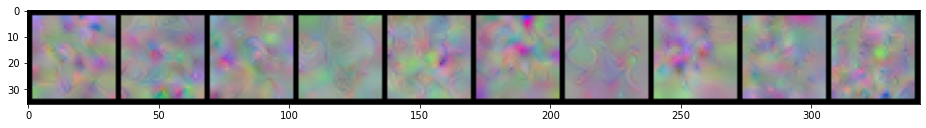
\includegraphics[width=\textwidth]{figures/INVERSION_CIFAR10_NN_0.png}



% \documentclass{article}
% \usepackage{graphicx}

% \ifluatex
%   \directlua{
%     tex.enableprimitives('', {'luaescapestring'})
%   }
%   \newcommand*{\Download}[2]{%
%     \IfFileExists{#1}{%
%     }{%
%       \directlua{
%         local io = require('io')
%         local http = require('socket.http')
%         local ltn12 = require('ltn12')
%         local file_name = '\luaescapestring{#1}'
%         local url = '\luaescapestring{#2}'
%         texio.write_nl('Downloading: ' .. file_name)
%         texio.write_nl('')
%         http.request{
%           url=url,
%           sink=ltn12.sink.file(io.open(file_name, 'w'))
%         }
%       }%
%     }%
%     \edef\DownloadFile{#1}%
%   }
% \else
%   \newcommand*{\Download}[2]{%
%     \IfFileExists{#1}{%
%     }{%
%       \immediate\write18{%
%         wget -O "#2" "#1"%
%       }%
%     }%
%     \edef\DownloadFile{#1}%
%   }%
% \fi

% \begin{figure}
% \centering
% \Download{profile-pics-16.jpg}{%
%     https://cdn.mos.cms.futurecdn.net/42E9as7NaTaAi4A6JcuFwG-970-80.jpg%
% }
% \includegraphics{\DownloadFile}
% \end{figure}